\section{Barbershop}
Il problema del Barbiere è formato da due tipi di processi, un processo barbiere che effettua tagli di barba/capelli a dei processi clienti, e un insieme di processi clienti che vogliono ricevere un taglio. Il negozio del barbiere prevede l'esistenza di una sala d'attesa con n-1 sedie, e la stanza del barbiere con una sedia dove viene effettuato il taglio, quindi in totale n sedie. Se non ci sono clienti che aspettano di essere serviti, il barbiere dorme. Se arriva un cliente nel negozio vi sono tre casi possibili; tutte le sedie sono occupate da altri clienti, e quindi il cliente se ne va dal negozio, oppure il barbiere è occupato e c'è almeno una sedia libera nella sala d'attesa, il cliente può sedersi ed aspettare che il barbiere si liberi ed effettui il taglio, infine se il barbiere sta dormendo, il barbiere si sveglierà e effettuerà il taglio al cliente.

É importante rispettare i seguenti vincoli:

\begin{itemize}
	\item I processi cliente dovrebbero ricevere il taglio;
	%\item Se un cliente arriva quando il negozio è pieno, se ne va;
	\item Il barbiere dovrebbe effettuare i tagli;
	\item Il barbiere serve i clienti uno per volta.
	
\end{itemize}

\subsection{Una possibile soluzione}
Il libro Little Book of Semaphores suggerisce la seguente soluzione: 

Sia n = 2, quindi una sedia per la sala d'attesa e una per la barberia. 

Si vuole utilizzare un \textsf{mutex} per proteggere la sezione critica al cui interno vi è un contattore di clienti presenti nel negozio. Quindi il contattore per essere modificato si dovrà garantire la mutua esclusione. Quando un cliente entra nel negozio dovrà entrare nella sezione critica per controllare che il contattore sia uguale a n, se lo è allora esce dal negozio, se invece non lo è incrementa il contattore ed esce dalla sezione critica. Una volta incrementato il cliente segnala attraverso un semaforo \textsf{Customer} la sua presenza al barbiere e si mette in attesa nel semaforo \textsf{Barber} per attendere il servizio del barbiere.

Una volta che il barbiere segnala la presa in carico del cliente sul semaforo \textsf{Barber}, viene effettuato il taglio e il cliente si sincronizza con il barbiere sui semafori \textsf{CustomerDone} e \textsf{BarberDone} per garantire che il taglio sia stato fatto, il barbiere poi può effettuare un taglio ad un altro cliente in attesa se c'è, altrimenti torna a dormire. Il cliente dopo il taglio entra di nuovo nella sezione critica per decrementare il contattore in modo tale da uscire dal negozio.

Il barbiere nello specifico all'inizio rimane in attesa sul semaforo \textsf{Customer} aspettando l'arrivo di un cliente ( simula il fatto che stia dormendo), una volta svegliato, segnala sul semaforo \textsf{Barber} di essere pronto con il taglio e prendere in carico un cliente(il primo che si sincronizza con il segnale), effettua il taglio e infine si sincronizza con il cliente che ha ricevuto il servizio. Se ci sono altri clienti in attesa passa direttamente al nuovo taglio senza mettersi a dormire, invece se non c'è nessuno torna a dormire e si ferma sul semaforo \textsf{Customer}.

\pagebreak
Di seguito viene mostrata una possibile soluzione in pseudo-codice.


\begin{figure}[h]
	\centering
	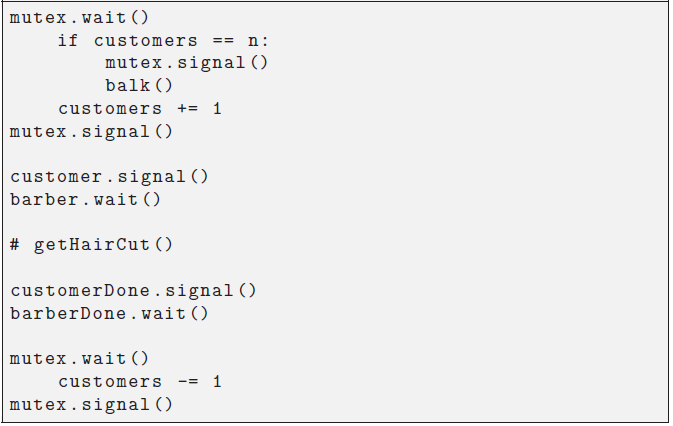
\includegraphics[width=0.6\textwidth]{Figure/2.png}
	\caption{Definizione processo cliente.}
%	\label{fig:baltdx}
\end{figure}

\begin{figure}[h]
	\centering
	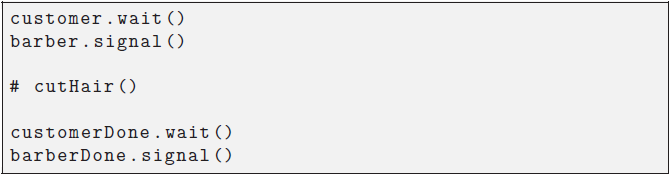
\includegraphics[width=0.6\textwidth]{Figure/3.png}
	\caption{Definizione processo barbiere.}
	%	\label{fig:baltdx}
\end{figure}
\subsection{Modellazione in CCS}

Quindi le entità utilizzate nel programma CCS sono:
\begin{itemize}
	\item \textsf{Customer$_{i}$}: Processo cliente che riceve il taglio;
	\item \textsf{Count$_{i}$}: \textsf{Mutex} con al suo interno il contattore del numero di clienti presenti nel negozio;
	\item \textsf{Barber}: Processo barbiere che effettua il taglio;
	\item \textsf{Sys}: Sistema.
\end{itemize}

Di seguito si mostra un esempio del sistema con n = 2 e tre clienti.

\textsf{Count1 = enter.incExit.Count2};\\
\textsf{Count2 = enter.(incExit.CountB + decExit.Count1)};\\
\textsf{CountB = enter.(balk.CountB + decExit.Count2)};\\

\textsf{Customer1 = 'enter.enter1.exit1.('incExit.C1 + 'balk.Customer1)};\\
\textsf{C1 = semCustomer.'semBarber.getHairCut1.semCustomerDone.'semBarberDone.\\'enter.enter1.exit1.'decExit.Customer1};\\

\textsf{Customer2 = 'enter.enter2.exit2.('incExit.C2 + 'balk.Customer2)};\\
\textsf{C2 = semCustomer.'semBarber.getHairCut2.semCustomerDone.'semBarberDone.\\'enter.enter2.exit2.'decExit.Customer2};\\

\textsf{Customer3 = 'enter.enter3.exit3.('incExit.C3 + 'balk.Customer3)};\\
\textsf{C3 = semCustomer.'semBarber.getHairCut3.semCustomerDone.'semBarberDone.\\'enter.enter3.exit3.'decExit.Customer3};\\

\textsf{Barber = 'semCustomer.semBarber.cutHair.'semCustomerDone.semBarberDone.Barber};

\textsf{set L = \{ enter, incExit, decExit, balk, semCustomer, semCustomerDone, semBarber, semBarberDone\}};

\textsf{Sys = (Customer1|Customer2|Customer3|Count1|Barber) \textbackslash L;}

\subsubsection{Codifica Mutex e contattore clienti}

Per codificare il contattore e il \textsl{mutex} si è deciso di utilizzare un unico processo, o meglio un insieme di processi che codificano il \textsf{mutex} e il contattore, perciò abbiamo: 

\textsf{Count1 = enter.incExit.Count2;}

Codifica il contattore che passa da zero a uno gestendo il tutto in mutua esclusione. Per interagire con il contattore i processi clienti devono sincronizzarsi su \textsf{enter} che risulta essere un canale ristretto, ciò permette la mutua esclusione che sarà dimostrata in seguito. Per poter incrementare il contattore e uscire dalla sezione critica i processi cliente utilizzeranno il canale \textsf{incExit} anch'esso ristretto, successivamente il processo \textsf{Count1} andrà nel processo \textsf{Count2} per mantenere il contattore a uno e per dare la possibilità di decrementare o incrementare un successivo processo cliente.

\textsf{Count2 = enter.(incExit.CountB + decExit.Count1);}

Codifica il contattore che passa da uno a due e/o da uno a zero, gestendo il tutto in mutua esclusione. Analogamente a \textsf{Count1} c'è \textsf{enter} per la sincronizzazione in mutua esclusione. Viene data una scelta in più su come proseguire l'esecuzione. A seconda di cosa richiede il processo cliente può essere data la possibilità di incrementare il contattore e uscire, sempre attraverso il canale \textsf{incExit}, oppure il decremento attraverso \textsf{decExit}(canale ristretto). La scelta dipende dello stato d'esecuzione in cui si trova il processo cliente. Nel caso incrementi, \textsf{Count2} passa a \textsf{CountB} altrimenti torna in \textsf{Count1}.

\textsf{CountB = enter.(balk.CountB + decExit.Count2);}

Codifica il contattore che non può essere più incrementato perché uguale a n e l'azione di decremento. Il funzionamento è uguale a \textsf{Count2} tranne per il fatto che \textsf{incExit} non esiste ma c'è \textsf{balk}(canale ristretto) usato per simulare l'uscita dal locale del cliente nel caso in cui voglia ricevere un taglio ma non ci sono sedie disponibili.

\subsubsection{Codifica Customer}

La codifica dei clienti avviene nel seguente modo:

\textsf{Customer1 ='enter.enter1.exit1.('incExit.C1 + 'balk.Customer1);}\\
\textsf{C1 = semCustomer.'semBarber.getHairCut1.semCustomerDone.'semBarberDone.}\\
\textsf{'enter.enter1.exit1.'decExit.Customer1;}

Il cliente per poter controllare se può entrare si sincronizza sul canale \textsf{enter} rimando in attesa della possibilità di entrare nella sezione critica. Una volta entrato controlla se può incrementare oppure no il contattore, quindi sceglie se eseguire \textsf{incExit} o \textsf{back}, tale scelta dipende da cosa offre il processo \textsf{count}. Nel caso sia \textsf{CountB}, l'unica azione possibile per il cliente è eseguire \textsf{balk} che lo fa uscire dalla sezione critica e non lo fa entrare nel negozio. Nel caso invece sia \textsf{Count1} o \textsf{Count2} il cliente esegue \textsf{incExit} cosi che incrementi il contattore e esca dalla sezione critica. Successivamente si sincronizza con il barbiere, che nel caso in cui il barbiere sia libero passa a ricevere il taglio. Finito il taglio si sincronizza subito con il barbiere per poi entrare nella sezione critica in mutua esclusione e decrementare il contattore per simulare la sua uscita dal negozio.

\subsubsection{Codifica Barber}

La codifica del Barbiere avviene nel seguente modo:

\textsf{Barber = 'semCustomer.semBarber.cutHair'semCustomerDone.semBarberDone.Barber;}

Il barbiere rimane in attesa di un nuovo cliente da servire su \textsf{semCustomer} se non ci sono cliente in attesa. Una volta arrivato un cliente si sincronizza con esso ed esegue il taglio, successivamente si sincronizza con il cliente appena servito per garantire che sia avvenuto il taglio per poi tornare all'inizio della sua esecuzione per poter eseguire un nuovo cliente se c'é, altrimenti attende un nuovo cliente.

\subsubsection{Codifica del sistema}

L'intero sistema viene codificato nel seguente modo:

\textsf{Sys = (Customer1|Customer2|Customer3|Count1|Barber) \textbackslash L;}\\
\textsf{set L = \{ enter, incExit, decExit, balk, semCustomer, semCustomerDone, semBarber, semBarberDone\};}

Il sistema viene rappresentato attraverso una composizione parallela dei processi \textsf{Customer, Barber e Count1}. Tutti i canali vengono ristretti per permettere la sincronizzazione dei processi, esclusi \textsf{cutHair, getHairCut$_{i}$, enter$_{i}$, exit$_{i}$} usati per mostrare un comportamento all'esterno.

\subsection{Verifica della correttezza attraverso CWB }

Di seguito si verificano se il programma definito rispetta tutte le caratteristiche stabilite dalla definizione del problema, attraverso l'uso della Edinburgh Concurrency Workbench (CWB).

\subsubsection{Trace Equivalence} 

Dato che il sistema con tre clienti e n = 2 risulta avere 752 stati, è troppo complesso scrivere una specifica che catturi il comportamento dell'intero sistema. Quindi trovare un specifica che sia bisimile a \textsf{Sys} non è molto interessante. Quello che ci interessa è perciò catturare alcune caratteristiche intessenti e utili per la verifica. Si procede quindi nello scrivere due specifiche generali che catturino, una la mutua esclusione nella modifica del contattore e l'altra che ogni cliente viene servito uno alla volta. Si hanno le seguenti:

\textsf{SpecM = enter1.exit1.SpecM + enter2.exit2.SpecM + enter3.exit3.SpecM;}

\textsf{SpecC = cutHair.getHairCut1.SpecC + getHairCut1.cutHair.SpecC + \\cutHair.getHairCut2.SpecC + getHairCut2.cutHair.SpecC + \\cutHair.getHairCut3.SpecC + getHairCut3.cutHair.SpecC;}

Si nota che unendo nel modo corretto queste due specifiche si può costruire la specifica bisimile a \textsf{Sys}, ma come detto risulta essere troppo complesso e quello che ci interessa è la cattura delle caratteristiche chiave del sistema, le quali garantiscono il corretto funzionamento.

Quindi si prendono due versioni di \textsf{Sys}, \textsf{Sys1} versione senza i canali \textsf{cutHair} e \textsf{getHairCut$_{i}$} e \textsf{Sys2} versione senza i canali \textsf{enter$_{i}$} e \textsf{exit$_{i}$}.

Per dimostrare che \textsf{Sys1} e \textsf{Sys2} hanno le caratteristiche descritte dalle specifiche \textsf{SpecM} e \textsf{SpecC} si ricorre all'uso della Trace Equivalence. Si vuole che le traccie di \textsf{Sys1} siano\textsf{ Tr(Sys1) = Tr(SpecM)}, mentre le traccie di \textsf{Sys2} siano \textsf{Tr(Sys2) = Tr(SpecC)}. \\
Vogliamo perciò che le traccie di \textsf{Sys1} siano sequenze di \textsf{enter$_{i}$} e \textsf{exit$_{i}$} ben accoppiate mentre per le traccie di \textsf{Sys2} siano sequenze di \textsf{cutHair} e \textsf{getHairCut$_{i}$} anch'essi ben accoppiate.

Attraverso la CWB con il commando \textbf{mayeq(Sys1,SpecM)} otteniamo la conferma che \textsf{Tr(Sys1) = Tr(SpecM)}. Analogamente con \textbf{mayeq(Sys2,SpecC)} si dimostra che \textsf{Tr(Sys2) = Tr(SpecC)}.

Si sottolinea che nonostante \textsf{Sys1} e \textsf{Sys2} hanno comportamenti esterni differenti, al loro interno sono garantite le due proprietà che si sono verificate con la Trace Equivalence, dato che si è solo modificato il comportamento esterno che ha origine dalla struttura interna del sistema rimasta in variata.

\subsubsection{Verifica tramite HML}

Passiamo ora a dimostrare alcune proprietà chiave del \textsf{Sys} attraverso la logica di Hennessy-Milner per una dimostrazione più formale.

Nelle verifiche verranno usate le seguenti formule:
\begin{itemize}
	\item \textbf{Inv(P)} = \textsf{max(X.(P \& [-]X));}\\
	Sempre vera la proprietà P.
	\item \textbf{Pos(P)} = \textsf{min(X. (P | <-> X));}\\
	Esiste un stato in cui vale la proprietà P.
	\item \textbf{WeakEven(P)} = \textsf{min(X. (P | <<eps>><-tau><<eps>>T \& [[eps]][-tau][[eps]] X )));}\\
	Prima o poi l'esecuzione eseguirà un stato in cui vale P attraverso passi interni e esterni.
	\item \textbf{WUntil(P,Q)} = \textsf{max(X. Q | (P \& [-]X));}\\
	Until in versione weak. Vale la proprietà P finché non diventa vera Q cioè l'esecuzione arriva un stato dove può vale Q.
	\item \textbf{SUntil(P,Q)} = \textsf{min(X. Q | (P \& <->T \& [-]X));}\\
	Until in versione strong. Vale la proprietà P finché non diventa vera Q.
\end{itemize}

\paragraph{Assenza di deadlock}\mbox{}

Il sistema riesce sempre a eseguire un passo senza rimanere bloccato.

\begin{center}
	\textsf{NoDeadlock = Inv(<->T);}
\end{center}

Con il commando \textbf{checkprop(Sys, Nodeadlock)} si ottiene \textbf{true}, quindi il sistema non va mai in deadlock.

\paragraph{Presenza di Livelock}\mbox{}

Siano:

\begin{center}
	\textsf{TauLoop = max (X. <tau> X);}\\
	\textsf{prop Livelock = Pos( TauLoop );}
\end{center}

Attreverso \textbf{checkprop(Sys, Livelock)} si ottiene \textbf{false}, quindi non vi è la presenza di Livelock.

\paragraph{Mutua esclusione contattore}\mbox{}

L'accesso alla sezione critica che contiene il contattore avviene in mutua esclusione, sia per incrementare e sia per decrementare il contattore (anche per eseguire \textsf{balk}). Quindi solo un processo può eseguire \textsf{exit} perché solo un processo cliente può trovarsi nella sezione critica.

\begin{center}
	\textsf{MutexC = Inv(
	([[exit1]]F | [[exit2]]F) \& 
 ([[exit2]]F | [[exit3]]F) \&
([[exit1]]F | [[exit3]]F));}
\end{center}

È sempre vero che al più solo uno dei tre processi è in grado di fare \textsf{exit$_{i}$}. Con il commando \textbf{checkprop(Sys, MutexC)} si ottiene \textbf{true}, quindi vale la mutua esclusione.

\paragraph{Mutua esclusione nell'esecuzione del taglio}\mbox{}

Ogni cliente viene servito uno alla volta, quindi non e possibile che due clienti vengono serviti contemporaneamente dal barbiere ma al più solo uno. Si dimostra perciò la mutua esclusione nell'esecuzione del taglio.

\begin{center}
	\textsf{MutexB = Inv(([[getHairCut1]]F | [[getHairCut2]]F) \& ([[getHairCut2]]F | [[getHairCut3]]F) \& ([[getHairCut1]]F | [[getHairCut3]]F));}
\end{center}

È sempre vero che al più solo uno dei tre processi è in grado di fare \textsf{getHairCut$_{i}$}. Con il commando \textbf{checkprop(Sys, MutexB)} si ottiene \textbf{true}, quindi vale la mutua esclusione.

%\paragraph{Verifica comportamento del cliente che entra quando il negozio pieno}\mbox{}

\paragraph{Verifica comportamento del barbiere nell'attesa dell'arrivo di un nuovo cliente }\mbox{}

Il barbiere aspetta, cioè dorme, finché non entra un cliente. Quindi a livello di codice CCS il processo \textsf{Barber} rimane fermo in \textsf{'semCustomer} finché non si sincronizza con un processo \textsf{Customer$_{i}$} attraverso l'azione \textsf{semCustomer}, dopo di che \textsf{Barber} può proseguire la sua esecuzione.

Per dimostrare tale proprietà si inseriscono nel sistema \textsf{Sys}, i canali \textsf{entered} in tutti i processi \textsf{C$_{i}$}, quindi:

\textsf{C1 = semCustomer.entered.'semBarber.getHairCut1.semCustomerDone.'semBarberDone.}\\
\textsf{'enter.enter1.exit1.'decExit.Customer1;}

Mentre nel processo \textsf{Barber} si inserisce \textsf{sleep} e \textsf{waked}, quindi:

\textsf{Barber = sleep.'semCustomer.waked.semBarber.cutHair.'semCustomerDone.semBarberDone.Barber;}

\begin{center}
	\textsf{UntilB = Inv([[sleep]]WUntil([[waked]]F, <<entered>>T));}
\end{center}

È sempre vero che in qualunque modo venga eseguito [[sleep]] è vero che il processo \textsf{Barber} non sa fare \textsf{waked} finché non diventa vero che un processo \textsf{Customer$_{i}$} può fare \textsf{entered}. La possibilità di poter fare \textsf{entered} la si ha solo se c'è stata una sincronizzazione, cioè il barbiere si è svegliato e il cliente è entrato e successivamente può segnalarlo. Quindi eseguendo \textbf{checkprop(Sys, UntilB)} si ottiene \textbf{true}, vale perciò la proprietà.

Non sarebbe andata bene la versione con lo strong until perché non è sempre vero in qualunque modo venga eseguito [[sleep]] è vero che il processo \textsf{Barber} non sa fare \textsf{waked} finché non diventa vero che un processo \textsf{Customer$_{i}$} esegue \textsf{entered}, infatti: 

\begin{center}
	 \textsf{UntilB = Inv([[sleep]]SUntil([[waked]]F, <<entered>>T));}
\end{center}

Allora \textbf{checkprop(Sys', UntilB)} ritorna \textbf{false}.
\pagebreak
\paragraph{Verifica comportamento del cliente nell'attesa di essere servito }\mbox{}

Il cliente aspetta, finché il barbiere non gli da il segnale di sedersi per il taglio. Quindi a livello di codice CCS il processo \textsf{Customer$_{i}$} rimane fermo in \textsf{'semBarber} finché non si sincronizza con un processo \textsf{Barber} attraverso l'azione \textsf{semBarber}, dopo di che \textsf{Customer$_{i}$} può proseguire la sua esecuzione.
\begin{center}
	\textsf{UntilC = Inv(WUntil([[getHairCut1]]F, <<cutHair>>T) \\| WUntil([[getHairCut2]]F, <<cutHair>>T) \\| WUntil([[getHairCut3]]F, <<cutHair>>T));}
\end{center}

È sempre vero che il processo \textsf{Customer$_{i}$} non sa fare \textsf{getHairCut$_{i}$} finché non diventa vero che il processo \textsf{Barber} può fare \textsf{cutHair}. La possibilità di poter fare \textsf{cutHair} la si ha solo se c'è stata una sincronizzazione. Si è aggiunta la clausola OR perché può accadere che nonostante si abbia la possibilità di poter fare \textsf{cutHair} non è detto che il processo \textsf{Customer$_{i}$} sa fare \textsf{getHairCut$_{i}$} perché a causa della mutua esclusione dopo la sincronizzazione, al più solo uno sa fare l'azione. Quindi eseguendo \textbf{checkprop(Sys, UntilC)} si ottiene \textbf{true}, vale perciò la proprietà.

\paragraph{Fairness}\mbox{}

Purtroppo la soluzione data al problema non garantisce una piena fairness, cioè può accadere che un processo \textsf{Customer$_{j}$} prenda per molte volte possesso del \textsf{Barber} lasciando gli altri processi \textsf{Customer$_{k\not=j}$} in attesa di un taglio. Vi è quindi solo garantita la possibilità che si possa ricevere il taglio.
Per dimostrare ciò si aggiunge ad ogni processo \textsf{Customer$_{i}$} il canale \textsf{will$_{i}$} per esprimere la volontà di effettuare un taglio dopo essersi seduto e per semplicità si tolgono i canali \textsf{enter$_{i}$} e \textsf{exit$_{i}$} (La mutua esclusione rimane garantita),quindi:

\textsf{C1 = will1.semCustomer.'semBarber.getHairCut1.semCustomerDone.'semBarberDone.}\\
\textsf{'enter.'decExit.Customer1;}

Sia la seguente formula:

\begin{center}
	\textsf{FairC = Inv([[will1]] Pos(<<getHairCut1>>T) \\\& [[[will2]] Pos(<<getHairCut2>>T) \\\& [[will3]] Pos(<<getHairCut3>>T)); }
\end{center}

Una volta espressa la volontà di eseguire un taglio esiste uno stato in cui è possibile effettuarlo. Quindi eseguendo \textbf{checkprop(Sys, FairC)} si ottiene \textbf{true}, esiste perciò uno stato in cui è possibile eseguire il taglio. Non è detto pero che venga eseguito questo, infatti:

\begin{center}
	\textsf{FairC2 = Inv([[will1]]WeakEven(<<getHairCut1>>T) \\\& [[will2]]WeakEven(<<getHairCut2>>T)) \\\& [[will3]]WeakEven(<<getHairCut3>>T)));}
\end{center}

È sempre vero che dopo aver espresso la volontà di eseguire un taglio attraverso \textsf{will$_{j}$} prima o poi il processo \textsf{Customer$_{j}$} lo riceverà. Ma per\textbf{ checkprop(Sys', FairC2)} risulta essere \textbf{false}, e quindi vale ciò che si è detto precedentemente, non vale la fairness.

Vi è garantita pero che non ci sia la possibilità di attesa infinita per ogni processo \textsf{Customer$_{i}$}, infatti siano:
\begin{center}
\textsf{WaitForever1 = max (X. <<getHairCut1>> X);}\\
\textsf{WaitForever2 = max (X. <<getHairCut2>> X);}\\
\textsf{WaitForever3 = max (X. <<getHairCut3>> X);}\\\mbox{}


\textsf{WaitForeverWill = (Pos(<<will1>> WaitForever1) | (Pos(<<will2>> WaitForever2)) | (Pos(<<will3>> WaitForever3)) );}
\end{center}

Attraverso \textbf{checkprop(Sys, WaitForeverWill)} si ottiene \textbf{false}, quindi non vi è la possibilità di avere attesa infinita nel ricevere il taglio.

Si può ragionare sul fatto che è possibile modificare il sistema in modo che sia garantita la fairness.

Una soluzione diciamo "semplice" può essere quella di far terminare i processi\textsf{Customer$_{i}$} una volta effettuato un taglio e quando sono terminati tutti, vi sia un processo preposto a riattivarli tutti. Questo modifica garantisce che prima o poi tutti i processi \textsf{Customer$_{i}$} eseguano un taglio.

Una soluzione migliore può essere quella di fermare i processi senza terminarli. Nello specifico si intende che quando un \textsf{Customer$_{j}$} riceve un taglio, per ricevere un nuovo taglio aspetta che tutti gli altri \textsf{Customer$_{k\in=j}$} ne ricevano almeno uno. Serve perciò un gruppo di processi in grado di capire come procede l'esecuzione e eseguire le giuste azione per garantire la fairness.

Quindi si aggiunge una nuova serie di processi che sono i seguenti:

\textsf{Sreset = 'sleep1.Sreset1 + 'sleep2.Sreset2 + 'sleep3.Sreset3;}\\
 \textsf{Sreset1 = 'sleep2.Sreset12-21 + 'sleep3.Sreset13-31;}\\
 \textsf{Sreset12-21 = 'sleep3.Wreset;} \\
 \textsf{Sreset13-31 = 'sleep2.Wreset; }\\
 \textsf{Sreset2 = 'sleep1.Sreset12-21 + 'sleep3.Sreset23-32;}\\
 \textsf{Sreset23-32 = 'sleep1.Wreset;} \\
 \textsf{Sreset3 = 'sleep1.Sreset13-31 + 'sleep2.Sreset23-32;}\\


 \textsf{Wreset = wakeUp1.Wreset23 + wakeUp2.Wreset13 + wakeUp3.Wreset12;}\\
 \textsf{Wreset23 = wakeUp2.Wreset3 + wakeUp3.Wreset2;}\\
 \textsf{Wreset13 = wakeUp1.Wreset3 + wakeUp3.Wreset1;}\\
 \textsf{Wreset12 = wakeUp1.Wreset2 + wakeUp2.Wreset1;}\\
 \textsf{Wreset1 =  wakeUp1.Sreset;}\\
 \textsf{Wreset2 =  wakeUp2.Sreset;}\\
 \textsf{Wreset3 =  wakeUp3.Sreset;}\\

Mentre vengono aggiunti i canali ristretti \textsf{sleep$_{i}$} e \textsf{wakeUp$_{i}$} ai processi \textsf{Customer$_{i}$}, quindi:

\textsf{C1 = will1.semCustomer.'semBarber.getHairCut1.semCustomerDone.'semBarberDone.\\'enter.'decExit.sleep1.'wakeUp1.Customer1;}

Il sistema diventa:

\textsf{Sys = (Customer1|Customer2|Customer3|Sreset|Count1|Barber) \textbackslash L;}

Quindi il funzionamento è il seguente:
Il processo \textsf{Customer$_{j}$} una volta terminato il taglio di sincronizza con \textsf{Sreset} attraverso \textsf{sleep$_{j}$} e per continuare poi deve sincronizzarsi anche con il processo \textsf{Wreset} attraverso \textsf{wakeUp$_{j}$}, ma questo è possibile solo se tutti gli altri \textsf{Customer$_{k\in=j}$} si sono sincronizzati con \textsf{Sreset} e quindi hanno ricevuto tutti lo stesso numero di tagli, allora a quel punto tutti i processi potranno ricevere un nuovo tagli sincronizzandosi prima con \textsf{Wreset} e ricominciando l'esecuzione.
Si sottolinea perciò che il processo \textsf{Sreset} e tutti i suoi sotto processi contiene tutte le possibili sequenze di sincronizzazione che i processi \textsf{Customer$_{i}$} fanno dopo aver ricevuto il taglio cosi che una volta completa una sequenza di sincronizzazione si ha la garanzia che tutti hanno ricevuto un taglio ciascuno. Analogamente il processo \textsf{Wreset} e tutti i suoi sotto processi contiene tutte le possibili sequenze di sincronizzazione per ricominciare l'esecuzione dei processi \textsf{Customer$_{i}$}.

Si può dimostrare che la fairness vale infatti ora,

\begin{center}
	\textsf{FairC2 = Inv([[will1]]WeakEven(<<getHairCut1>>T) \\\& [[will2]]WeakEven(<<getHairCut2>>T)) \\\& [[will3]]WeakEven(<<getHairCut3>>T)));}
\end{center}

Con \textbf{checkprop(Sys', FairC2)} risulta essere vera.


